\documentclass[tikz,border=3pt]{standalone}
\usepackage{tikz}
\usetikzlibrary{arrows.meta,positioning,fit,shapes.geometric}
\definecolor{blue}{HTML}{4C78A8}
\definecolor{orange}{HTML}{F58518}
\definecolor{green}{HTML}{54A24B}
\tikzset{
box/.style={draw=black!45,rounded corners=2pt,align=center,minimum height=8mm,
  text width=29mm,font=\small,fill=white},
gate/.style={diamond,draw=black!45,align=center,aspect=2.2,font=\small,fill=black!3},
arr/.style={-{Latex[length=2mm]},thick,draw=black!65},
note/.style={font=\scriptsize,align=center,text=black!70}
}
\begin{document}
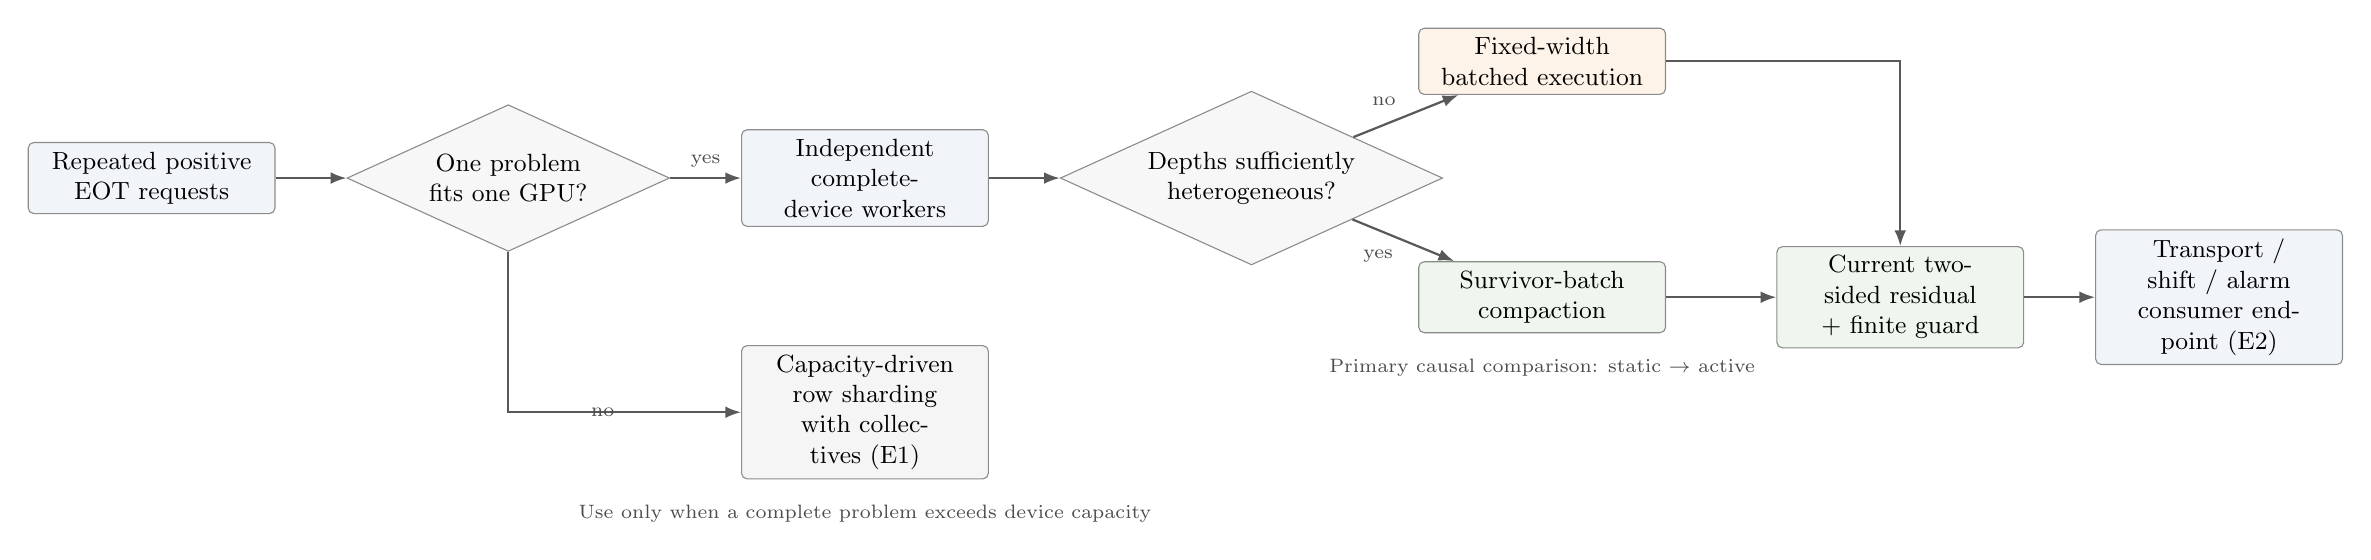
\begin{tikzpicture}[node distance=7mm and 9mm]
\node[box,fill=blue!8] (stream) {Repeated positive\\EOT requests};
\node[gate,right=of stream] (fit) {One problem\\fits one GPU?};
\node[box,right=of fit,fill=blue!8] (workers) {Independent complete-\\device workers};
\node[gate,right=of workers] (depth) {Depths sufficiently\\heterogeneous?};
\node[box,above right=5mm and 9mm of depth,fill=orange!10] (static) {Fixed-width\\batched execution};
\node[box,below right=5mm and 9mm of depth,fill=green!10] (active) {Survivor-batch\\compaction};
\node[box,below=15mm of workers,fill=black!4] (shard) {Capacity-driven row sharding\\with collectives (E1)};
\node[box,right=14mm of active,fill=green!10] (verify) {Current two-sided residual\\+ finite guard};
\node[box,right=of verify,fill=blue!8] (consumer) {Transport / shift / alarm\\consumer endpoint (E2)};
\draw[arr] (stream) -- (fit);
\draw[arr] (fit) -- node[note,above]{yes} (workers);
\draw[arr] (fit) |- node[note,left,pos=.75]{no} (shard);
\draw[arr] (workers) -- (depth);
\draw[arr] (depth) -- node[note,above left]{no} (static);
\draw[arr] (depth) -- node[note,below left]{yes} (active);
\draw[arr] (static.east) -| (verify.north);
\draw[arr] (active) -- (verify);
\draw[arr] (verify) -- (consumer);
\node[note,below=2mm of active] {Primary causal comparison: static $\rightarrow$ active};
\node[note,below=2mm of shard] {Use only when a complete problem exceeds device capacity};
\end{tikzpicture}
\end{document}
